% Title: Report LaTex File: Literature Review
% Auther: DC Eksteen
% Student Number: 22623906
% Contact: 22623906@sun.ac.za
% Date: 2022/09/17
% Version: 2.1

\chapter{Literature Review}
% Overview of the focus of the lietrature review:

% Plan for Literature Review Layout:
% Zwift: Technology and Requirements
% Existing Trainer Technology
% Bluetooth Technology
% Bicycle Specifications
% Eddy Current Brake
% Sensor Technology

The literature review is performed to define the requirements for the connection with Zwift, as well as discovering and understanding the various desired and required features and products that exist on the market today.

\section{Overview}

\newpage

\section{Zwift: Technology and Requirements}

As mentioned above, Zwift uses real-time training data to drive the avatar in the virtual world. In order to achieve this, Zwift needs to run on a device that has :

\begin{itemize}
	\item An internet connection to connect to the Zwift servers via the \ac{api}.
	\item \ac{ble} or ANT+ functionality to receive the data from the training session.
\end{itemize}

This device is usually a laptop, mobile phone or tablet, and will also display the avatar in the virtual world to the player. Moving forward, this device will be referred to as the "host" device as it is the central device controlling the user experience. \citep{Bromley:2022}

\subsection{Basic Requirements}
As mentioned above, Zwift requires real-time tracking data from the player in order to control the avatar. The interactiveness and accuracy of the experience greatly depends on the amount and nature of the data that is sent to the host device (also sometimes referred to as the 'main unit').

\begin{table}[h!]
	\renewcommand{\arraystretch}{1.5}
	\centering
	\begin{tabularx}{0.8\textwidth}{ p{3cm} X}
		\toprule
		Requirement  & Impact                                                                                                                   \\
		\midrule
		Speed data   & Most basic data requirement and is essential to the use of the Zwift platform.                                           \\
		Cadence data & Not essential for platform, but a feature that many players prefer to have available.                                    \\
		Power data   & Not essential for platform, although it is the preferred metric that Zwift will use to measure the effort of the player. \\
		\bottomrule
	\end{tabularx}
\end{table}

\subsection{\ac{ble} vs ANT+}
Both \ac{ble} and ANT+ devices communicate using \ac{uhf} electromagnetic waves with frequencies around \SI{2.4}{\giga\hertz}. The communication also takes part over a small distance.

\subsubsection{\ac{ble} for Fitness Devices}
\ac{ble} is one of two standards for Bluetooth communication that has been developed and maintained by \ac{bsig}.\footnote{The other being Bluetooth \ac{bbr}}The specific details of the technology and standard is discussed in Section \ref{sec:ble}. For the sake of Zwift requirements, this section will look at the specific protocol of the \ac{ble} specification that Zwift supports.\\
In the past, when Zwift was just launched, all of the Bluetooth communication was performed using proprietary protocols provided by the manufacturers of trainers and training equipment as there has not yet been a standard protocol defined to handle Bluetooth communication of controllable sports equipment. \\
On 14 February 2017, \ac{bsig} adopted the \ac{ftms} protocol to the \ac{ble} \ac{gatt}. Then, in late 2021 Zwift announced that they will be supporting \ac{ftms} in their latest update, and thus any new trainer that would like to interact with the Zwift platform would be required to follow the \ac{ftms} protocol as is discussed in Section \ref{sec:ftms}. \citep{Jeremy:2021}\\
Table \ref{tab:blreq} below shows the different commands within the \ac{ftms} protocol that Zwift uses to control connected trainers. This can be deducted from the control modes that are available on the platform, and have been confirmed by a Zwift engineer on the official support forums.

\begin{table}[H]
	\renewcommand{\arraystretch}{1.5}
	\centering
	\caption{Zwift Supported \ac{ftms} Commands}
	\begin{tabularx}{0.8\textwidth}{ >{\raggedright}p{4cm} X}
		\toprule
		Command                              & Description                                                               \\
		\midrule
		Set Target Resistance Level          & Sends the desired resistance level to the trainer.                        \\
		Set Target Power                     & Sends the targeted power (Watts) that the trainer should aim to maintain. \\
		Start or Resume                      & Starts or resumes a training session on the trainer                       \\
		Stop or Pause                        & Stop or pause a training session on the trainer.                          \\
		Set Indoor Bike Simulation Parameter & Set the simulation parameters on the trainer                              \\
		\bottomrule
	\end{tabularx}
	\label{tab:blreq}
\end{table}

Depending on the type of workout that is being performed, Zwift will use the different control point commands listed in Table \ref{tab:blreq} above. When the user is normally riding around within the Zwift world, it will send \ac{sim} parameter commands. This is explained in more detail in Section \ref{sec:sim}. When the user is using the "Workout Mode", Zwift has the option to engage "ERG" mode, where it will send a desired power target that the trainer should aim to maintain regardless of the speed. Thus the user can decide to go faster, with the trainer lowering the resistance, or go slower with the trainer having an increased resistance. Lastly, the user can adjust the resistance on their trainer from within the Zwift software, requiring Zwift to then send that specific command to the trainer.

\newpage

\section{Existing Trainer Technology}


\section{\ac{ble} Communication}
\label{sec:ble}
\ac{ble} works by forming pico - and scatter-net networks between various master and slave devices. Each device in the network is either a master or a slave, but never both. The devices then form a piconet when one or more slaves connect and synchronize with a single master device. The role of the master device is then to manage the slave devices through the protocol. This forms a network as can be seen in Figure \ref{fig:ble} below.\\

\begin{figure}[H]
	\begin{center}
		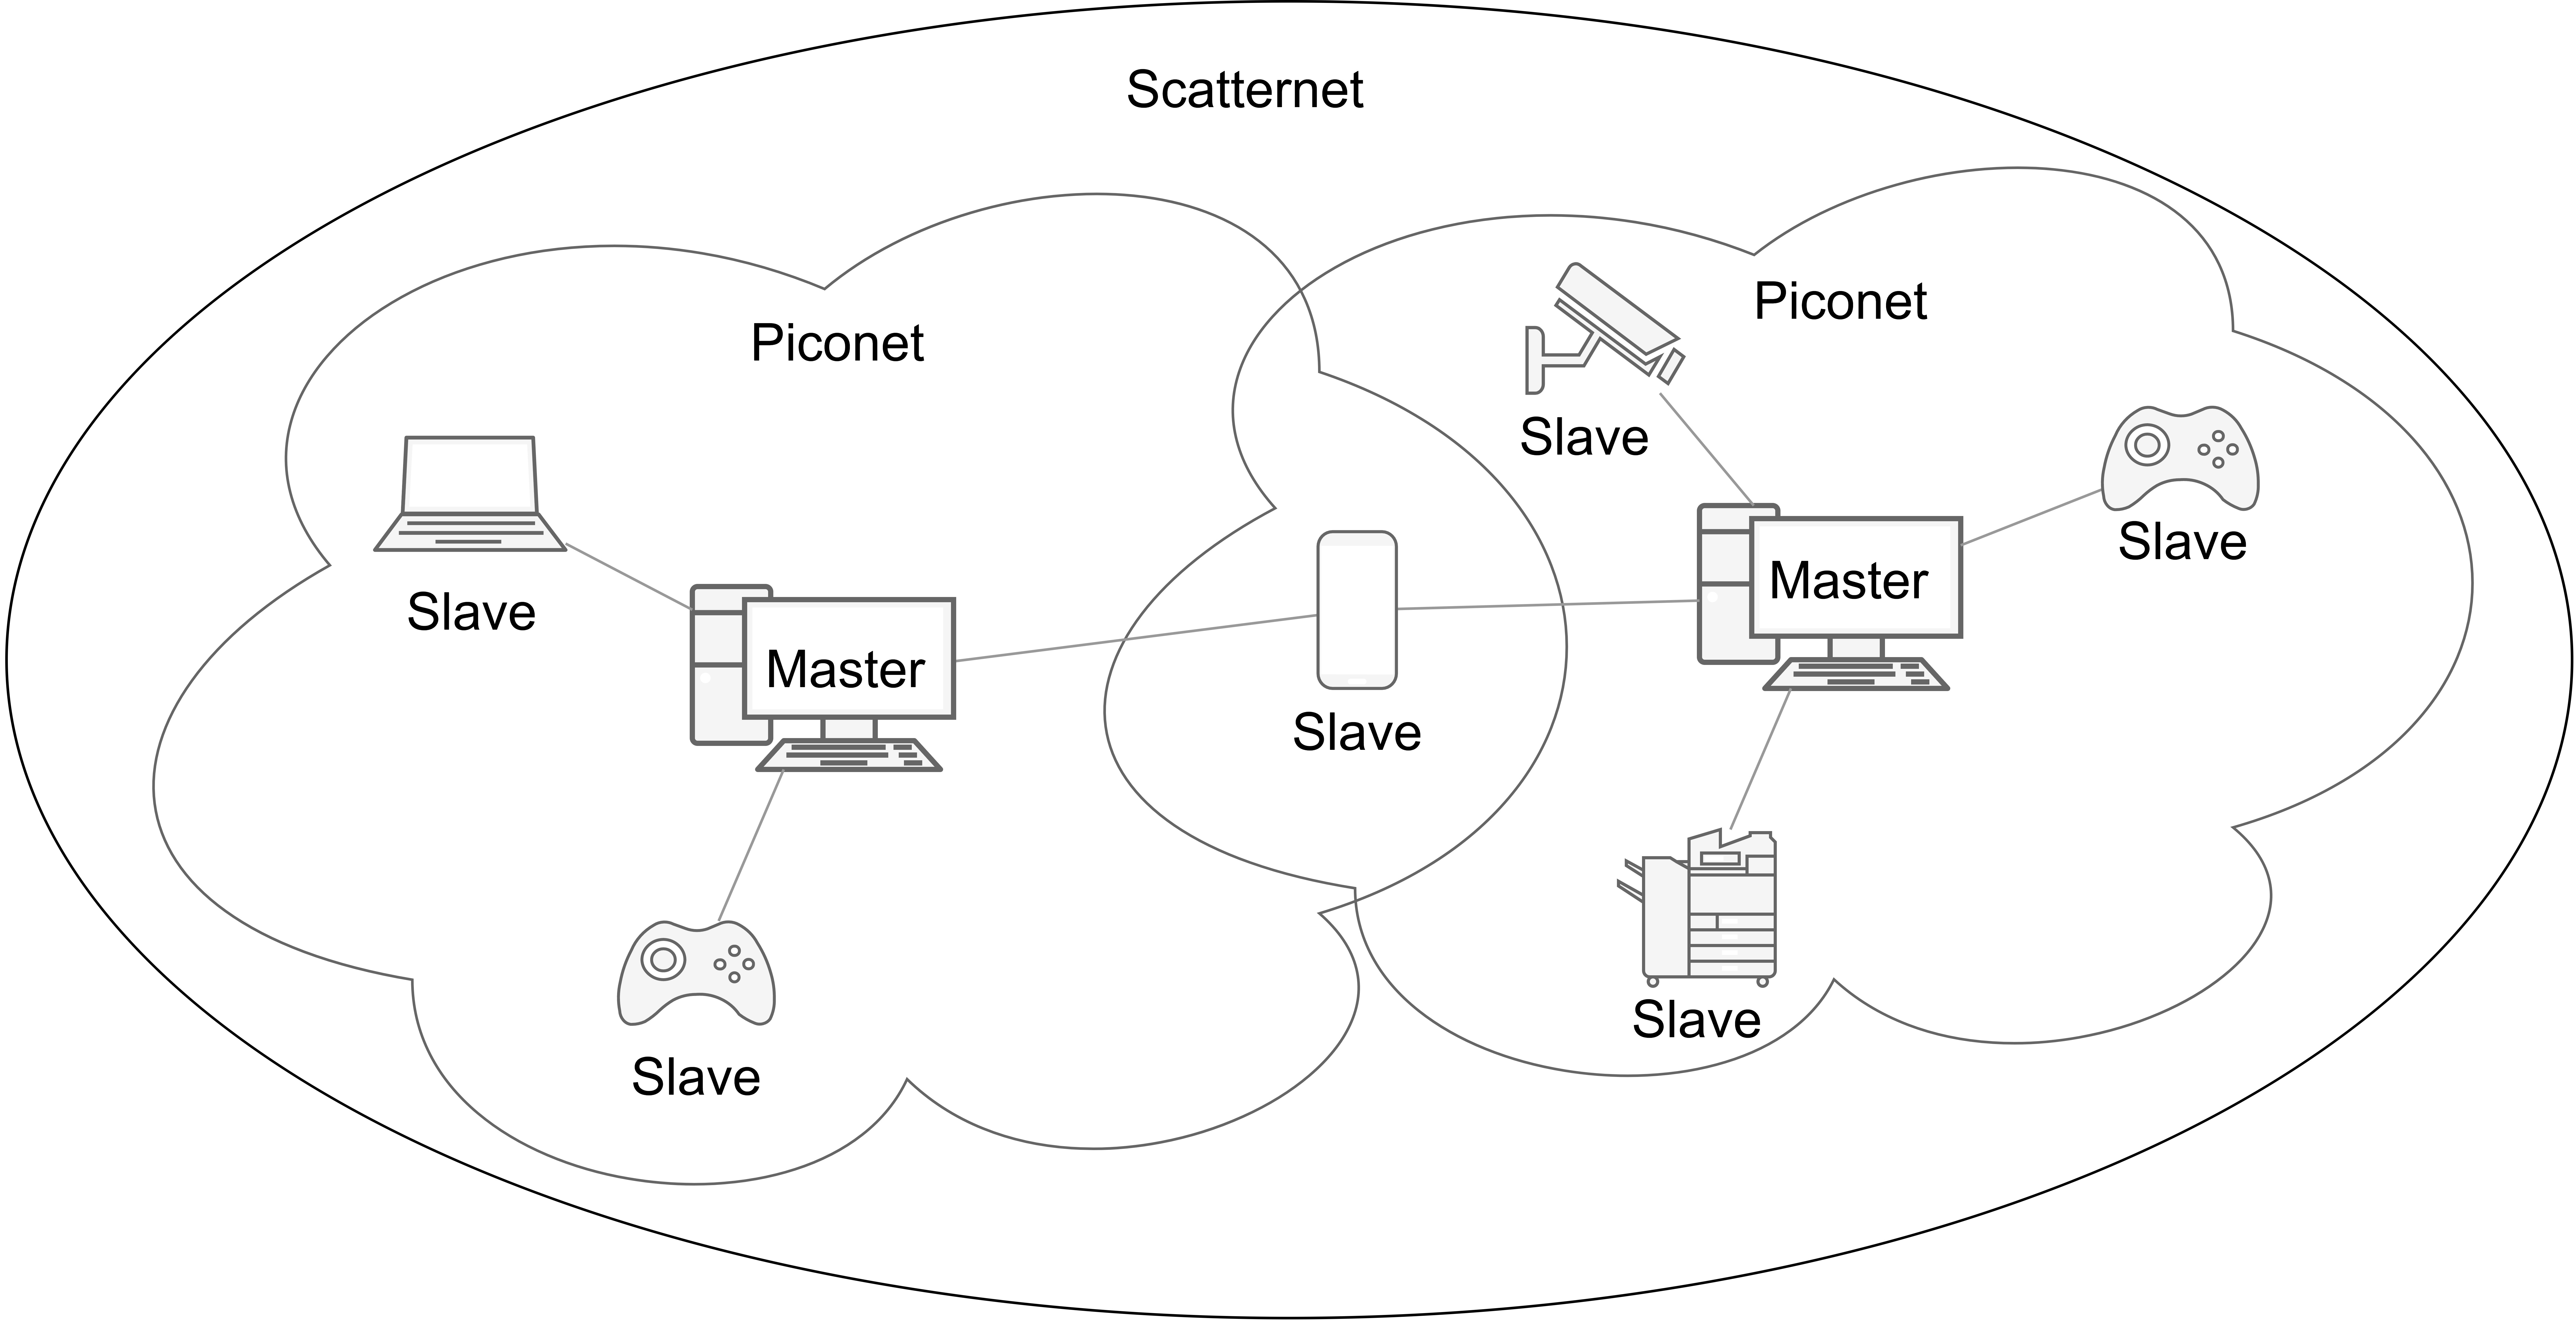
\includegraphics[width=0.9\textwidth]{BLEnet.jpg}
		\caption{\ac{ble} Star Network Topology}
		\label{fig:ble}
	\end{center}
\end{figure}

The master thus determines how often a slave is allowed to communicate, and slaves only communicate when requested to do so by a master. This is with one exception in the case of "advertising". Advertising is a feature that allows a slave device to announce that it has something to transmit to the master. This is either an event message or a measurement value.
\newpage
Some other features worth considering are listed in Table \ref{tab:ble} below:
\begin{table}[H]
	\renewcommand{\arraystretch}{1.5}
	\centering
	\caption{Technical Specifications of the \ac{ble} Standard}
	\begin{tabularx}{0.9\textwidth}{>{\raggedright}p{2.5cm} >{\raggedright}p{3cm} >{\raggedright\arraybackslash}X}
		\toprule
		Description        & Specification                       & Detail                                                                                                                                                 \\
		\midrule
		Data Package Size  & 64 bit (min) to 216 bit (max)       & The size of any single data package that can be sent between a master and slave(s).                                                                    \\
		Data Transfer Rate & \SI{1}{Mbps}                        & The rate at which the data is typically transferred between devices.                                                                                   \\
		Security           & 128-bit AES                         & Security and encryption varies in levels, but generally data is encrypted between devices with a "shared secret" key that is generated during pairing. \\
		Latency            & \SI{6}{\milli\second}               & Time between device starting transmission and data getting transferred. (Aka network lag).                                                             \\
		Power Consumption  & \SI{0.01}{\watt} to \SI{0.5}{\watt} & The power required by a device to join and operate on the piconet.                                                                                     \\
		\bottomrule
	\end{tabularx}
	\label{tab:ble}
\end{table}

\subsubsection{\ac{ftms} Protocol}\label{sec:ftms}
Within the \ac{ftms} protocol, there is a sub-protocol dedicated to Indoor Bike Data that focuses specifically on the application of the protocol for bike trainers. \cite[section ~4.9]{BLSIG:2017}.\\
The specification outlines and defines services that are supported by the protocol. Table \ref{tab:ftmsft} and \ref{tab:ftmstg} below lists the available features that are of interest to the project. Machine Features are Parameters that can be requested from the trainer, and Target Features are training parameters that can be set from an external device. \citep{BLSIG:2017}

\begin{minipage}{\textwidth}
	\begin{table}[H]
		\renewcommand{\arraystretch}{1.2}
		\centering
		\caption{Relevant Optional Fitness Machine Features of \ac{ftms} Protocol}
		\begin{tabularx}{\textwidth}{p{1.4cm} >{\raggedright}p{5cm} >{\raggedright\arraybackslash}X}
			\toprule
			Number                                                & Feature                          & Description                                                                          \\
			\midrule
			NA\footnote{This feature is compulsory for protocol.} & Instantaneous Speed              & Trainer can determine the instantaneous speed of the user.                           \\
			0                                                     & Average Speed Supported          & Trainer can determine the average speed of the user for the duration of the session. \\
			1                                                     & Cadence Supported                & Trainer can determine pedalling rate of the user (rpm).                              \\
			7                                                     & Resistance Level Supported       & Trainer can determine the resistance the user experiences.                           \\
			10                                                    & Heart Rate Measurement Supported & Trainer is able to determine the heart rate of the user.                             \\
			14                                                    & Power Measurement Supported      & Trainer is able to determine the power generated by the user.                        \\
			\bottomrule
		\end{tabularx}
		\label{tab:ftmsft}
	\end{table}
\end{minipage}

The parameters that would be relevant to the control of a bicycle trainer connected to Zwift are listed in Table \ref{tab:ftmstg} below:
\begin{table}[H]
	\renewcommand{\arraystretch}{1.2}
	\centering
	\caption{Relevant Optional Target Setting Features of \ac{ftms} Protocol}
	\begin{tabularx}{\textwidth}{p{1.4cm} >{\raggedright}p{5cm} >{\raggedright\arraybackslash}X}
		\toprule
		Number & Feature                    & Description                                             \\
		\midrule
		1      & Inclination Target Setting & Trainer can adjust difficulty to simulate inclination.  \\
		2      & Resistance Target Setting  & Trainer can adjust resistance level.                    \\
		3      & Power Target Setting       & Trainer can adjust difficulty to maintain power target. \\
		13     & \ac{sim} Parameters        & Trainer supports \ac{sim} mode.                         \\
		\bottomrule
	\end{tabularx}
	\label{tab:ftmstg}
\end{table}

\subsubsection{\ac{sim} mode}
\label{sec:sim}

This mode is defined in the \ac{ftms} documentation, and needs Control Permission to be activated. Once the mode is activated, the trainer will receive parameter arrays with the data shown in Table \ref{tab:sim} below to determine the required resistance level.

\begin{table}[H]
	\renewcommand{\arraystretch}{1.3}
	\centering
	\caption{\ac{sim} Mode Parameter Data}
	\begin{tabularx}{0.8\textwidth}{>{\raggedright\arraybackslash}X >{\centering\arraybackslash}p{1cm} >{\raggedleft\arraybackslash}p{2cm}}
		\toprule
		Parameter                             & Size   & Resolution \\
		\midrule
		Wind Speed (\SI{}{\meter\per\second}) & 16 bit & 0.001      \\
		Grade (\SI{}{\percent})               & 16 bit & 0.01       \\
		\ac{crr}                              & 8 bits & 0.0001     \\
		\ac{cw} (\SI{}{\kilogram\per\meter})  & 8 bits & 0.01       \\
		\bottomrule
	\end{tabularx}
	\label{tab:sim}
\end{table}

The \textit{Grade} indicates the gradient of the road that the avatar is travelling on. The \text{\ac{crr}} is determined by the road surface and wheel type of the avatar in the game, where the \textit{\ac{cw}} is determined by the player's weight and height, and can then be reduced by in-game events such as equipment selection and drafting behind other avatars when this feature is active. Currently Zwift does not utilize the \textit{Wind Speed} parameter.\\
These parameters are then used by the trainer to determine the resistance required to simulate the conditions in the game. This is what creates the realistic training experience.

\section{Bicycle Specifications}
% Section showing expected bicycle specifications of most popular models
The two most common types of bicycles that are expected to be used on the trainer are \acp{mtb} and road bicycles. The dimensions that are relevant to the implementation of the trainer are the wheelbase, wheel diameter and weight, as shown in Figure \ref{fig:bikeDim} below.

\begin{figure}[H]
	\centering
	\begin{subfigure}{.5\textwidth}
		\centering
		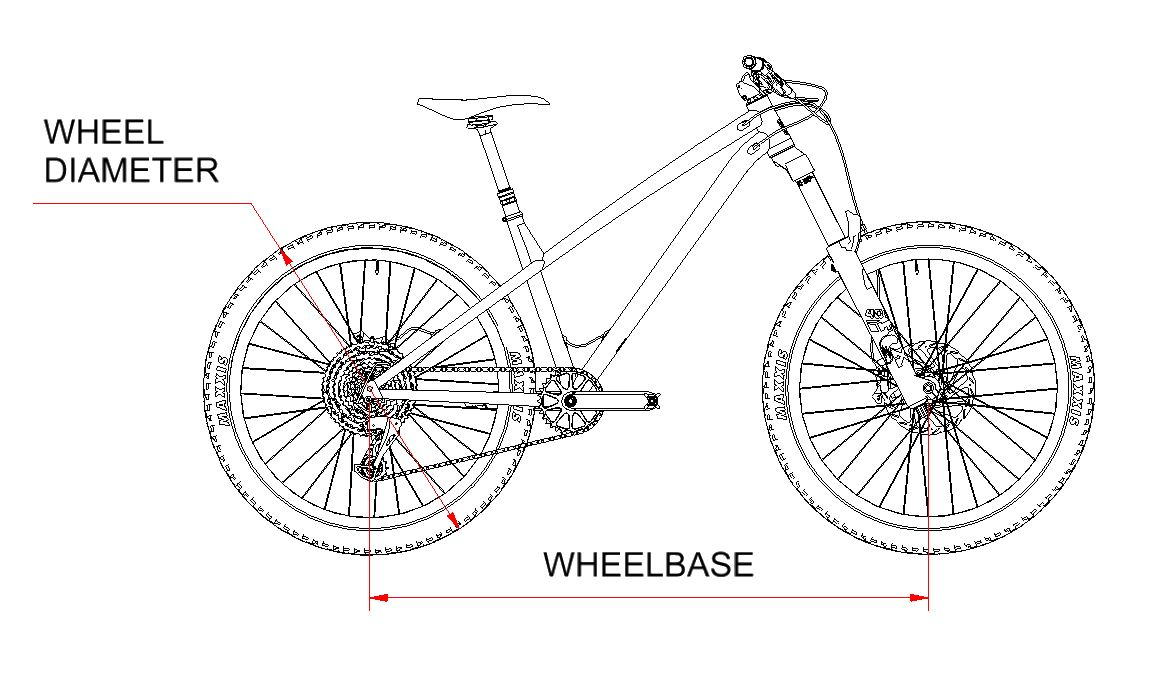
\includegraphics[width=\linewidth]{measureMTB.jpg}
		\caption{\ac{mtb} \citep[model by:][]{Pratama:2021}}
		\label{fig:sub1}
	\end{subfigure}%
	\begin{subfigure}{.5\textwidth}
		\centering
		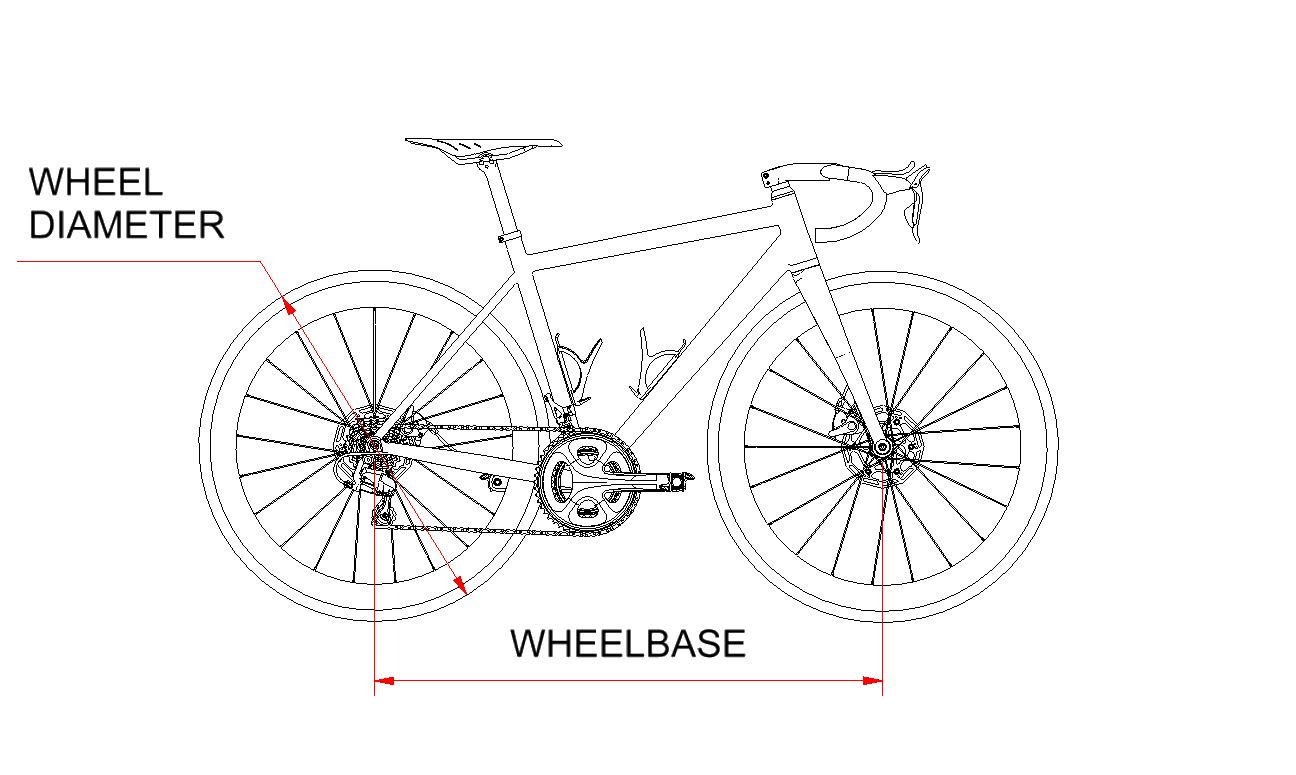
\includegraphics[width=\linewidth]{measureRoad.jpg}
		\caption{Road Bicycle \citep[model by:][]{Morozev:2017}}
		\label{fig:sub2}
	\end{subfigure}
	\caption{Bicycle Dimensions}
	\label{fig:bikeDim}
\end{figure}

Although these dimensions vary between brands, models and sizes, a general overview of common dimensions can be found by comparing the largest and smallest size dimensions from the best selling models in each category, as well as the average size that can be expected. The best selling bike models for each category are shown with their dimensions in Table X below: \citep{Lin:2021}

\begin{table}[H]
	\renewcommand{\arraystretch}{1.2}
	\centering
	\caption{Best selling road bicycle specifications}
	\begin{tabularx}{\textwidth}{p{2.6cm} X Xp{0.05cm} p{2.6cm} X X}
		\toprule
		Road Bike           & \multicolumn{2}{c}{Wheelbase} &                         & \ac{mtb} & \multicolumn{2}{c}{Wheelbase}                                                     \\
		                    & Smallest                      & Largest                 &          &                               & Smallest                & Largest                 \\
		\midrule
		Specialized Tarmac  & \SI{969}{\milli\meter}        & \SI{1012}{\milli\meter} &          & Specialized Epic              & \SI{1116}{\milli\meter} & \SI{1211}{\milli\meter} \\
		Specialized Roubaix & \SI{981}{\milli\meter}        & \SI{1024}{\milli\meter} &          & Trek Fuel EX                  & \SI{1144}{\milli\meter} & \SI{1323}{\milli\meter} \\
		Cervelo R3          & \SI{971}{\milli\meter}        & \SI{1024}{\milli\meter} &          & Specialized Stumpjumper       & \SI{1152}{\milli\meter} & \SI{1302}{\milli\meter} \\
		\bottomrule
	\end{tabularx}
	\label{tab:bikes}
\end{table}

\section{Eddy Current Brake}
% Section on Eddy Current Brake
\section{Sensor Technology}
% Rotary Encoder
\section{Conclusion}
% Section summerizing the literature review
